\section{Project Summary}
This section contains an explanation of what Willy is meant to do, how the current project will work towards that goal, and to what ends.

Willy started its life as a concept for a garbage collecting robot, meant to drive autonomously through the city center in Zwolle.
For a few years the project continued with that as a goal, until Hogeschool Windesheim and TAoR (The Art of Robotics) went their separate ways \cite{taor}.
The project is now run solely by Windesheim.
According to the previous group, there is still some ongoing discussion about who truly owns the project, but for the sake of simplicity the assumption will be made Willy solely belongs to Windesheim.

After this falling out, Willy got a new purpose in its robotic life, as a robotic greeter.
The goal of Willy is now no longer to drive around and remind people to throw away their garbage neatly, but instead drive around and inform people about public events at Windesheim.

For the current project, this does not matter much.
The goal of this semester of Future Technology for Willy is to improve the autonomous driving to the point where the April tags (located on the ceiling of various points in T5) are no longer needed.

Initially, the assumption was made that these were used as key points in navigation for Willy, but after a very informative meeting with the previous group, it was revealed that the only reason these tags still exist is to use as calibration points and setting an easy target for Willy to navigate to.
This means that the scope of the project is slightly shifted.
As such, the key focus is on lessening the standard PID controller feedback swing (as illustrated in figure \ref{fig::pid}.

\begin{figure}[H]
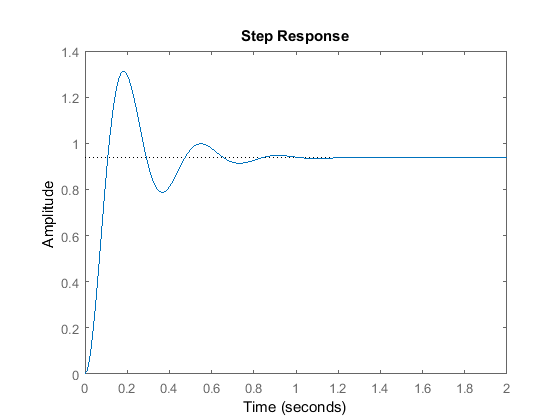
\includegraphics[width=12cm]{pidgraph.png}
\caption{A rough demonstration of PID correction}
\label{fig::pid}
\end{figure}

By reducing the amount of corrections needed by the navigation stack \cite{navstack}, the "Drunken Polish Driving" effect, as described by one of the previous project groups, can be lessened.
This would mean a smoother autonomous driving experience.
\newpage